The Timit corpus \cite{timit} was used for verifying the proposed solution. It contains recordings of 630 speakers from 8 different regions in the united states. Each speaker read 10 sentences, recorded at 16 KHz frequency. Beside the audio recordings, the corpus contains time-aligned orthographic, word and phonetic transcription.\\\\
To create the spectrogram images that are used as input to our phone recognition network, the phonetic time alignment information are used to extract the frames associated with each phoneme. The frames of each phoneme are then split into 16ms Hanning windows with 15.5 ms overlap. A Fast Fourier Transform is then applied on the frames to generate a spectrogram, which are then padded to create a 128 by 128 pixels images. Figures \ref{fig:spec1} and \ref{fig:spec2} shows example spectrograms.
\begin{figure}[H]
\centering
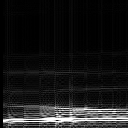
\includegraphics[width=0.6\linewidth]{figs/ao.png}
\caption{Spectrogram of phoneme \textbf{ao}}
\label{fig:spec1}
\end{figure}
\begin{figure}[H]
\centering
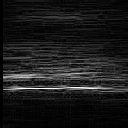
\includegraphics[width=0.6\linewidth]{figs/sh.png}
\caption{Spectrogram of phoneme \textbf{sh}}
\label{fig:spec2}
\end{figure}